
\chapter{Design}
\section{Actors}
The application involves three primary categories of actors, each with distinct roles and permissions:
\begin{itemize}
	\item \textit{Non-Authenticated User (Guest User):} refers to an anonymous individual who accesses the application without logging in. This actor is allowed to register, authenticate using existing credentials, or explore the platform by searching for doctors and viewing their public profiles.
	
	\item \textit{Patient (User):} represents the end-user of the service. Once authenticated, the patient can book appointments with doctors, confirm or cancel them, and subsequently provide feedback through reviews.
	
	\item \textit{Doctor:} a professional figure who offers medical appointments. The doctor can manage their availability schedule, making it accessible to patients, and consult an analytics dashboard displaying aggregated data such as earnings, reviews, and the number of visits performed.
\end{itemize}

\section{Functional Requirements}
The following section outlines the functional requirements.

\subsection{Guest Users}
\textbf{Guest users} are allowed to:
\begin{itemize}
	\item Register for an account within the application;
	\item Log in using their credentials;
	\item Initiate the password recovery process in case of forgotten credentials;
	\item Search for doctors and access their public profiles.
\end{itemize}

\subsection{Patients}
Authenticated users identified as \textbf{patients} are granted the following capabilities:
\begin{itemize}
	\item Manage and update their personal profiles;
	\item Search for doctors and access their public profiles;
	\item Book appointments and optionally include a note for the doctor;
	\item Endorse a doctor as a form of support or recommendation;
	\item Submit reviews regarding their medical experience;
	\item View their appointments, including past, current, and upcoming ones;
	\item Search for doctors through the recommendation feature provided by the system.
\end{itemize}

\subsection{Doctors}
Authenticated users identified as \textbf{doctors} are provided with the following functionalities:
\begin{itemize}
	\item Manage and update their personal and professional profiles;
	\item Search for other doctors and access their public profiles;
	\item Define and configure the types of visits offered, along with the associated pricing;
	\item Oversee appointments by identifying scheduled patients and appointments for the current day;
	\item Configure and manage appointment availability through customizable scheduling templates;
	\item Monitor and respond to patient reviews;
	\item Access analytics, including visual representations of revenue, newly acquired patients, recent reviews, and a summary of completed visits.
\end{itemize}

\section{Non-Functional Requirements}
The following non-functional requirements address the quality attributes of the system, ensuring its performance, reliability, security, scalability, and maintainability.

\subsection{Performance and Scalability}
\begin{itemize}
	\item The system shall maintain \textbf{acceptable response times} for common operations such as viewing medical records and scheduling appointments; 
	\item The system shall efficiently \textbf{handle increased workload} during peak usage periods without degradation of service.
\end{itemize}

\subsection{Availability and Reliability}
\begin{itemize}
	\item The application shall be \textbf{available} to all users \textbf{24/7}, minimizing downtime through redundancy and failover mechanisms;
	\item The system shall implement \textbf{backup and recovery procedures} to preserve data integrity and support rapid restoration after failures.
	\item The system shall tolerate occasional data staleness in non-critical views, ensuring high availability even under degraded conditions.
\end{itemize}

\subsection{Security and Privacy}
\begin{itemize}
	\item The system shall enforce \textbf{secure, authenticated access for all users}, employing strong password policies and session management;
	\item All sensitive data shall be encrypted both in transit and at rest;
	\item The system provides defenses against injections. 
\end{itemize}

\subsection{Usability}
\begin{itemize}
	\item The user interface shall be intuitive and \textbf{user‑friendly}, enabling users to perform tasks with minimal learning curve.
	\item The application shall exhibit \textbf{low latency} in user interactions to maintain a responsive experience.
\end{itemize}

\subsection{Portability and Flexibility}
\begin{itemize}
	\item The application shall be \textbf{deployable on multiple operating systems} (e.g., Windows, macOS, Linux) without requiring behavioral changes.
	\item The system’s architecture shall support the addition of new attributes or modules (e.g., new appointment types) with minimal code modification.
\end{itemize}

\subsection{Maintainability}
\begin{itemize}
	\item The codebase shall follow \textbf{Object-Oriented design} principles, promoting modularity and ease of comprehension.
	\item The system shall \textbf{minimize single points of failure} through component decoupling and redundancy.
	\item The application shall include comprehensive documentation and code comments to facilitate future enhancements and debugging.
\end{itemize}

\section{Use Case Diagram}

\begin{figure}[H]
    \centering
	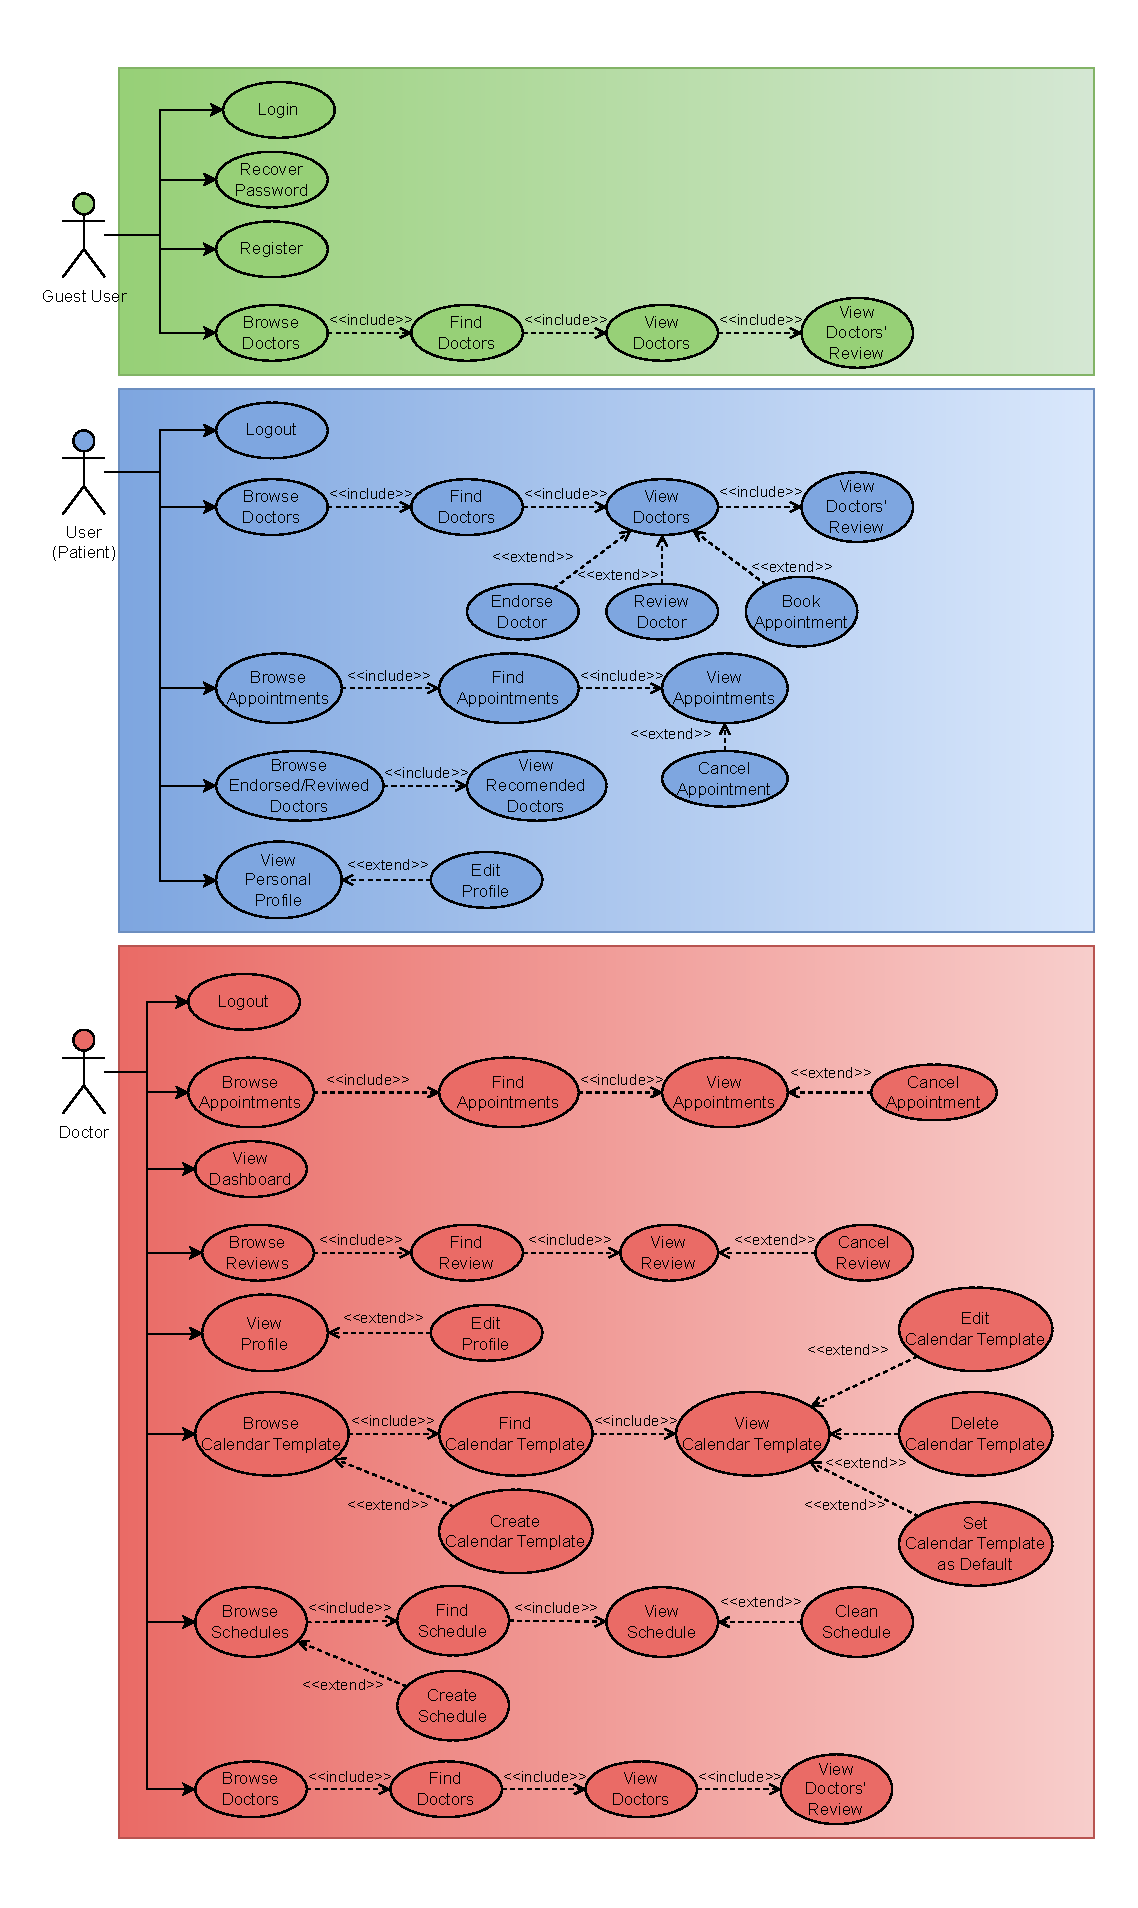
\includegraphics[scale=0.60]{./resources/healthhub_use_case.pdf}
    \caption{Use Case Diagram for HealthHub}
    \label{fig:use-case-diagram}
\end{figure}

The use case diagram illustrates the core functionalities of the \textit{HealthHub} application, categorized by the actors involved: \textit{Guest}, \textit{User (Patient)}, and \textit{Doctor}. The Guest actor can access basic features such as registration, login, and browsing doctors. The authenticated user (Patient) can view and edit their profile, search for doctors, view doctor reviews, book and cancel appointments, endorse or review doctors, and receive personalized recommendations. The Doctor actor has access to a personal dashboard from which they can manage their schedule, define and edit calendar templates, view appointments, delete reviews, and handle their availability. Use cases are modeled with \texttt{<<include>>} and \texttt{<<extend>>} relationships to reflect functional modularity and reuse of common interactions like viewing profiles or appointments.


\section{UML Class Diagram}

\begin{figure}[!h]
    \centering
	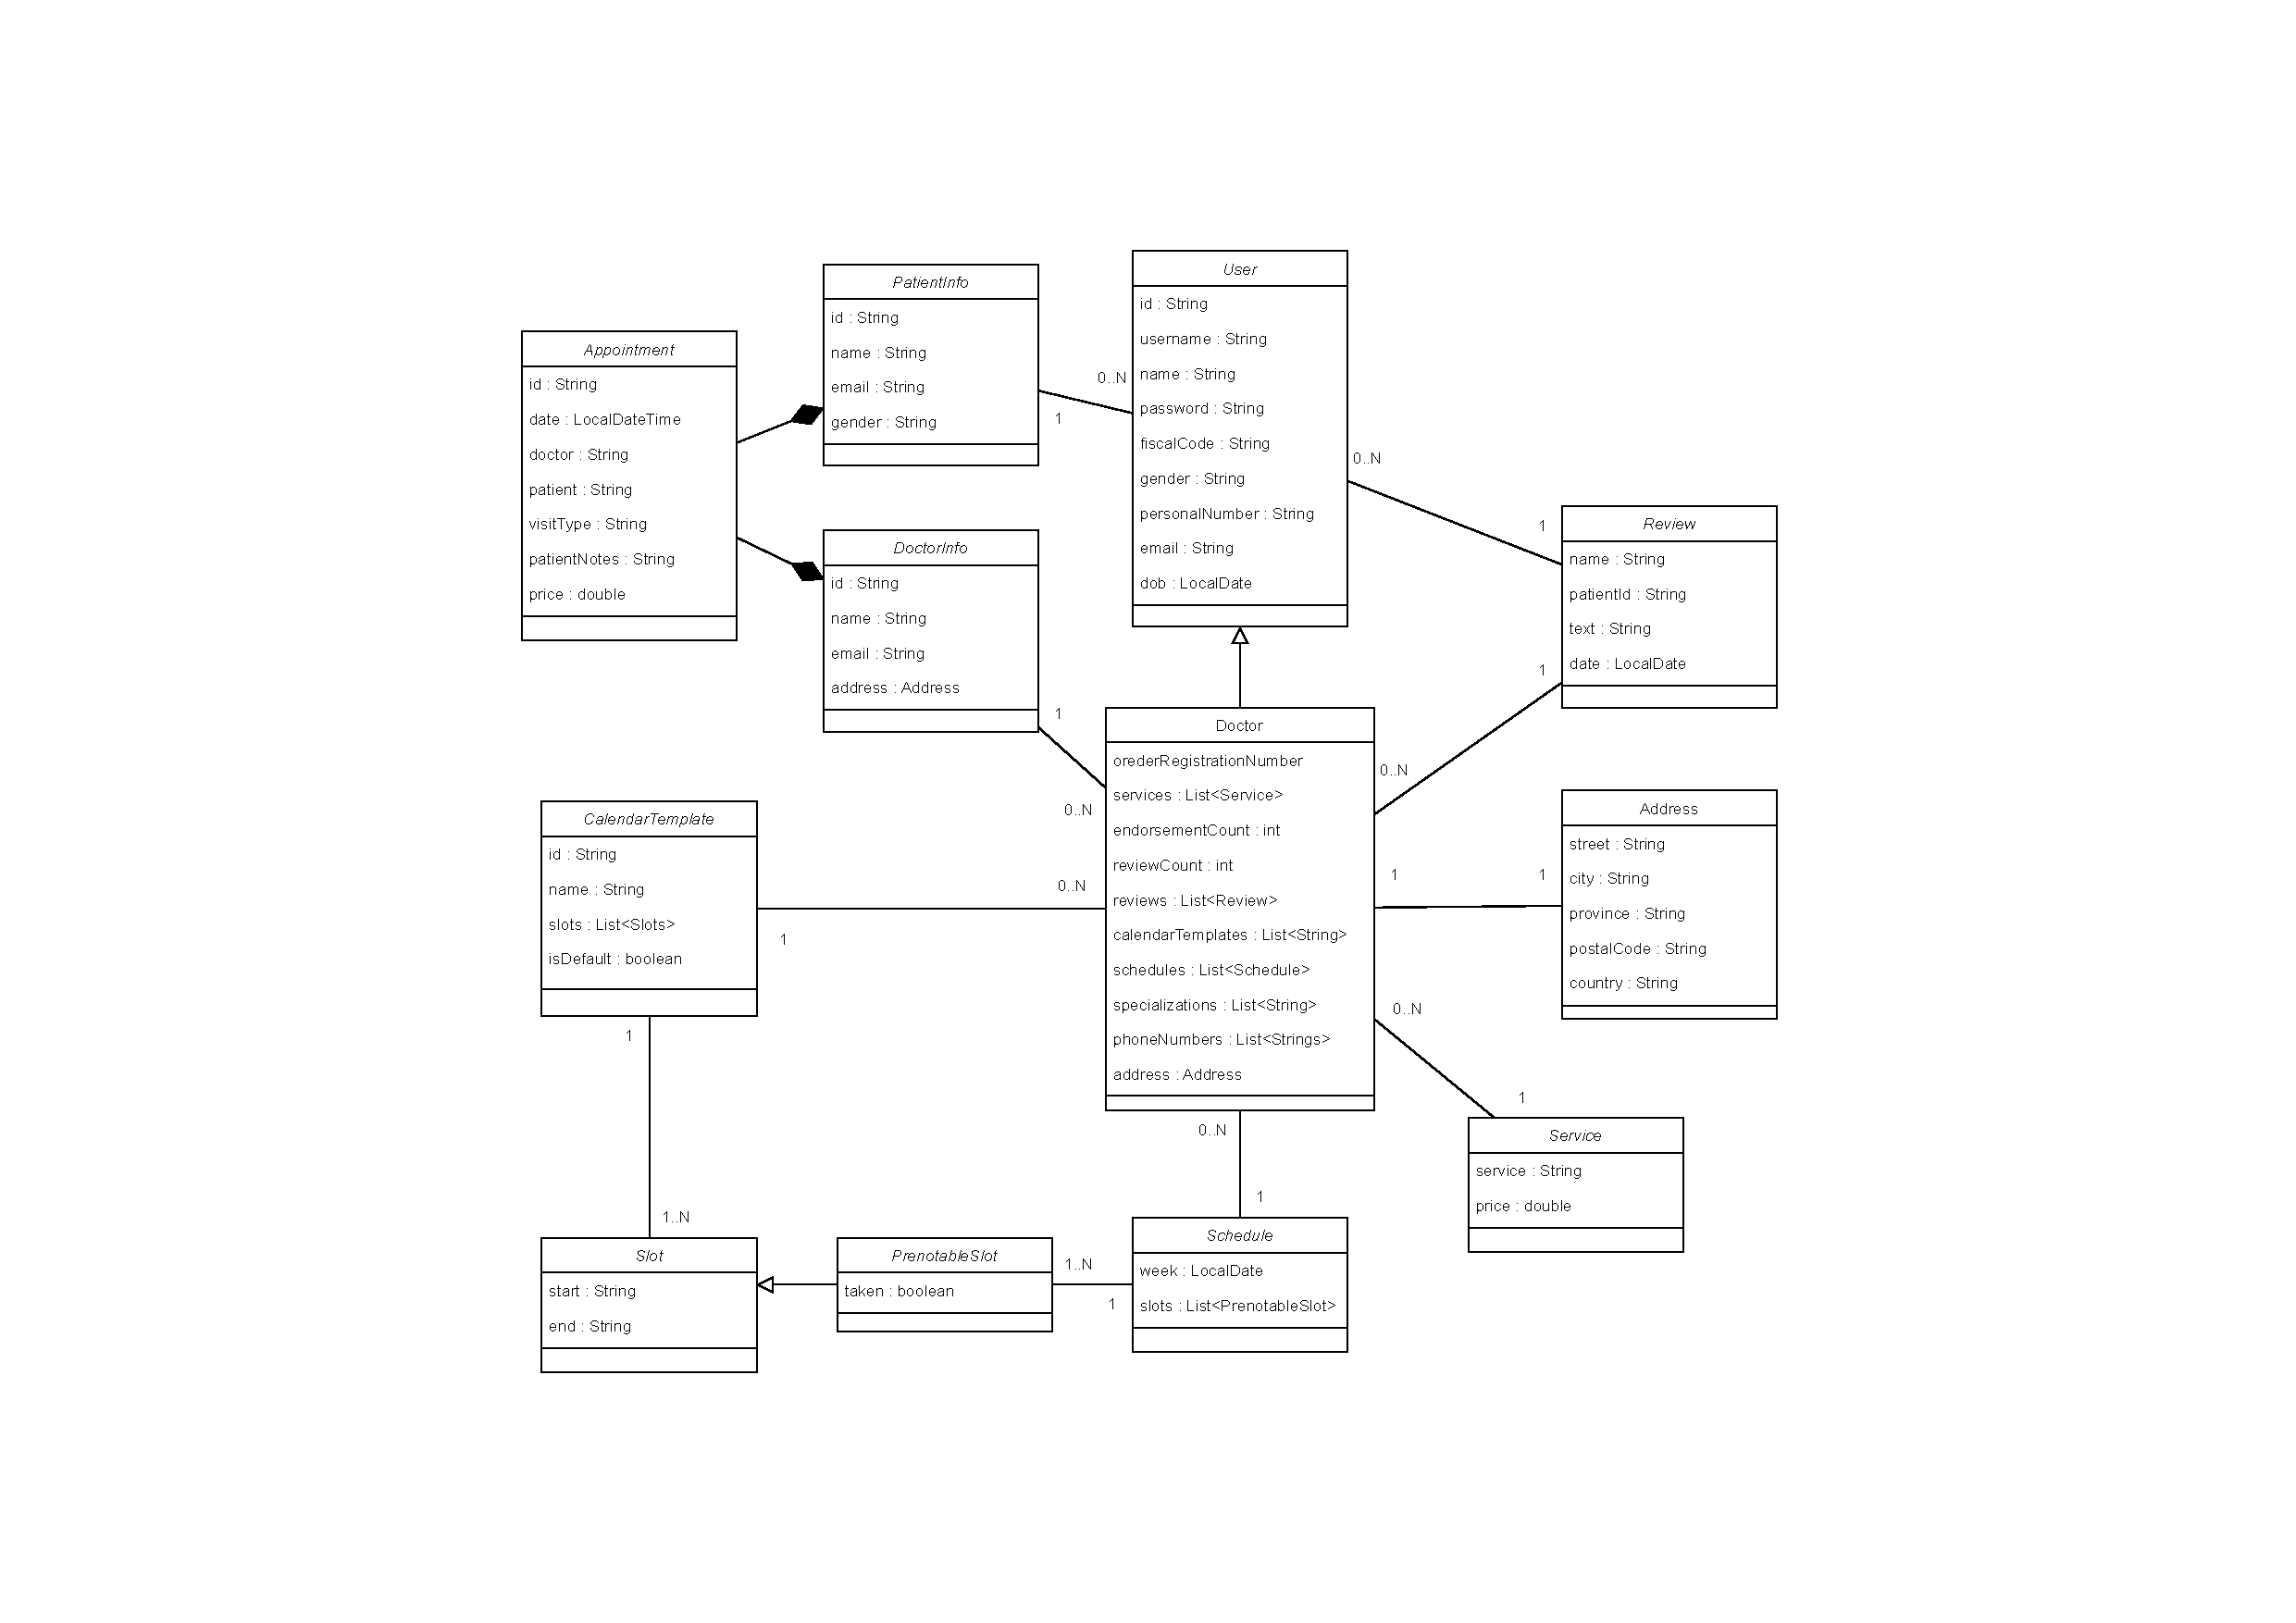
\includegraphics[scale=0.69]{./resources/healthhub_UML.pdf}
    \caption{UML Class Diagram for HealthHub}
    \label{fig:uml-diagram}
\end{figure}

\subsection{Relationships between classes}
Here we briefly summarise the relation between each class.
\begin{itemize}
	\item \textbf{Doctor} is a specialization of \textbf{User};
	\item A \textbf{Doctor} may offer zero or more \textbf{Service} instances and each \textbf{Service} is provided by exactly one \textbf{Doctor};
	\item A \textbf{Doctor} may have zero or more \textbf{Review} entries and each \textbf{Review} refers to exactly one \textbf{Doctor}; 
	\item A \textbf{Doctor} may define zero or more \textbf{CalendarTemplates} and each \textbf{CalendarTemplate} belongs to exactly one \textbf{Doctor};
	\item A \textbf{Doctor} may publish zero or more \textbf{Schedules} and each \textbf{Schedule} is associated with exactly one \textbf{Doctor};
	\item Each \textbf{Schedule} comprises zero or more \textbf{PrenotableSlots} and each \textbf{PrenotableSlot} is part of exactly one \textbf{Schedule};
	\item Each \textbf{CalendarTemplate} comprises zero or more \textbf{Slots} and each \textbf{Slot} belongs to exactly one \textbf{CalendarTemplate}; 
	\item A \textbf{Doctor} has exactly one \textbf{Address} and each \textbf{Address} is linked to exactly one \textbf{Doctor} (and similarly to \textbf{DoctorInfo}); 
	\item An \textbf{Appointment} is associated with exactly one \textbf{DoctorInfo} and one \textbf{PatientInfo} and each \textbf{DoctorInfo} or \textbf{PatientInfo} may have zero or more \textbf{Appointments}. 
\end{itemize}

\subsection{Design of the classes}
Here we briefly summarise the primary attributes of each entity.

\begin{description}
	\item[\textbf{User}] 
	\hfill
	\begin{itemize}
		\item \texttt{id: String} – unique identifier  
		\item \texttt{username: String}  
		\item \texttt{name: String}  
		\item \texttt{password: String} – stored as hash  
		\item \texttt{fiscalCode: String}  
		\item \texttt{gender: String}  
		\item \texttt{personalNumber: String}  
		\item \texttt{email: String}  
		\item \texttt{dob: LocalDate}  
	\end{itemize}

	\item[\textbf{Doctor}] (specialization of \textbf{User}) 
	\hfill
	\begin{itemize}
		\item \texttt{orderRegistrationNumber: String}  
		\item \texttt{services: List<Service>}  
		\item \texttt{endorsementCount: int}  
		\item \texttt{reviewCount: int}  
		\item \texttt{reviews: List<Review>}  
		\item \texttt{calendarTemplates: List<CalendarTemplate>}  
		\item \texttt{schedules: List<Schedule>}  
		\item \texttt{specializations: List<String>}  
		\item \texttt{phoneNumbers: List<String>}  
		\item \texttt{address: Address}  
	\end{itemize}
	
	\item[\textbf{Address}]
	\hfill
	\begin{itemize}
		\item \texttt{street: String}  
		\item \texttt{city: String}  
		\item \texttt{province: String}  
		\item \texttt{postalCode: String}  
		\item \texttt{country: String}  
	\end{itemize}
	
	\item[\textbf{Appointment}]
	\hfill
	\begin{itemize}
		\item \texttt{id: String}  
		\item \texttt{date: LocalDateTime}  
		\item \texttt{visitType: String}  
		\item \texttt{patientNotes: String}  
		\item \texttt{price: double}  
	\end{itemize}
	
	\item[\textbf{Schedule}]
	\hfill
	\begin{itemize}
		\item \texttt{week: LocalDate}  
		\item \texttt{slots: List<PrenotableSlot>}  
	\end{itemize}

	\item[\textbf{CalendarTemplate}]
	\hfill
	\begin{itemize}
		\item \texttt{id: String}  
		\item \texttt{name: String}  
		\item \texttt{slots: List<Slot>}  
		\item \texttt{isDefault: boolean}  
	\end{itemize}
	
	\item[\textbf{Slot}]
	\hfill
	\begin{itemize}
		\item \texttt{start: String}  
		\item \texttt{end: String}  
	\end{itemize}
	
	\item[\textbf{PrenotableSlot}] (subclass of \textbf{Slot})
	\hfill
	\begin{itemize}
		\item \texttt{taken: boolean}  
	\end{itemize}
	
	\item[\textbf{Review}]
	\hfill
	\begin{itemize}
		\item \texttt{name: String}  
		\item \texttt{patientId: String}  
		\item \texttt{text: String}  
		\item \texttt{date: LocalDate}  
	\end{itemize}
	
	\item[\textbf{Service}]
	\hfill
	\begin{itemize}
		\item \texttt{service: String}  
		\item \texttt{price: double}  
	\end{itemize}
	
	\item[\textbf{PatientInfo}] (belong to \textbf{Appointment})
	\hfill
	\begin{itemize}
		\item \texttt{id: String}  
		\item \texttt{name: String}  
		\item \texttt{email: String}  
		\item \texttt{gender: String}  
	\end{itemize}
	
	\item[\textbf{DoctorInfo}] (belong to \textbf{Appointment})
	\hfill
	\begin{itemize}
		\item \texttt{id: String}  
		\item \texttt{name: String}  
		\item \texttt{email: String}  
		\item \texttt{address: Address}  
	\end{itemize}
\end{description}
